\chapter*{Le Kerala de Cochin à Munnar\markboth{Le Kerala de Cochin à Munnar}{}}
\section*{8 novembre 2015}
J'atteris à Cochin, sur la côte ouest au sud de l'Inde \newline
 Visite de Fort Kochi, ancienne ville coloniale hollandaise, célèbre pour ses filets de pêche chinois \newline
 \newline
\centerline{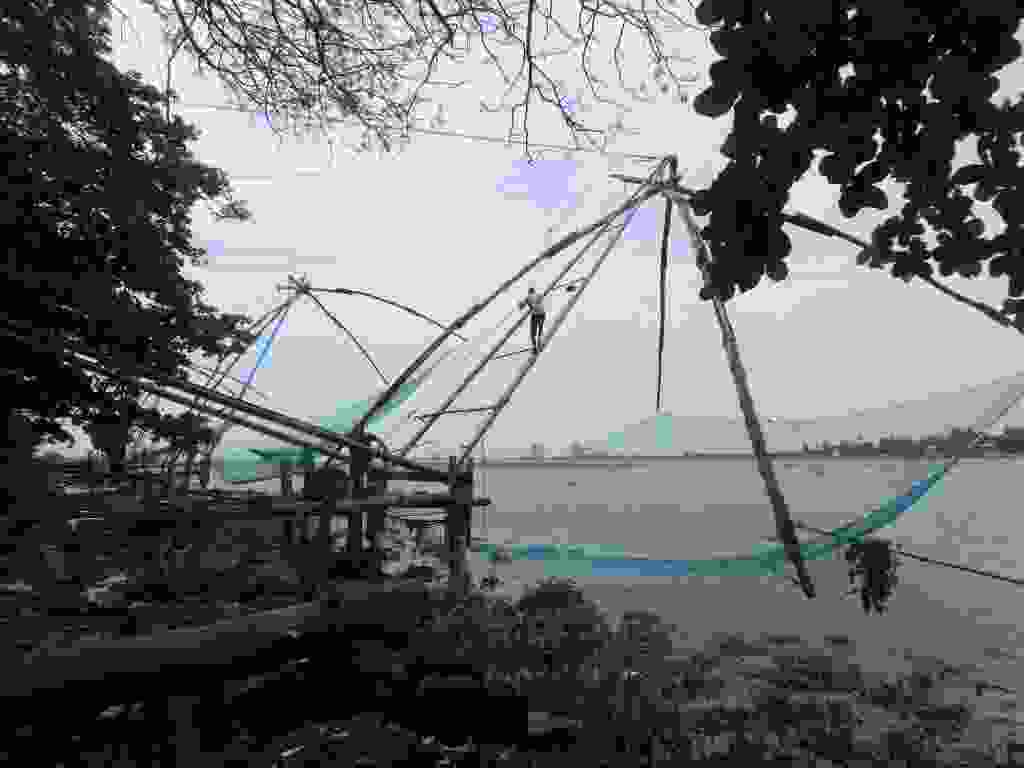
\includegraphics[width=\mywidth]{../wp-content/uploads/2015/11/wpid-oi000179-1024x768.jpg} } 
 \newline
 \newline
\centerline{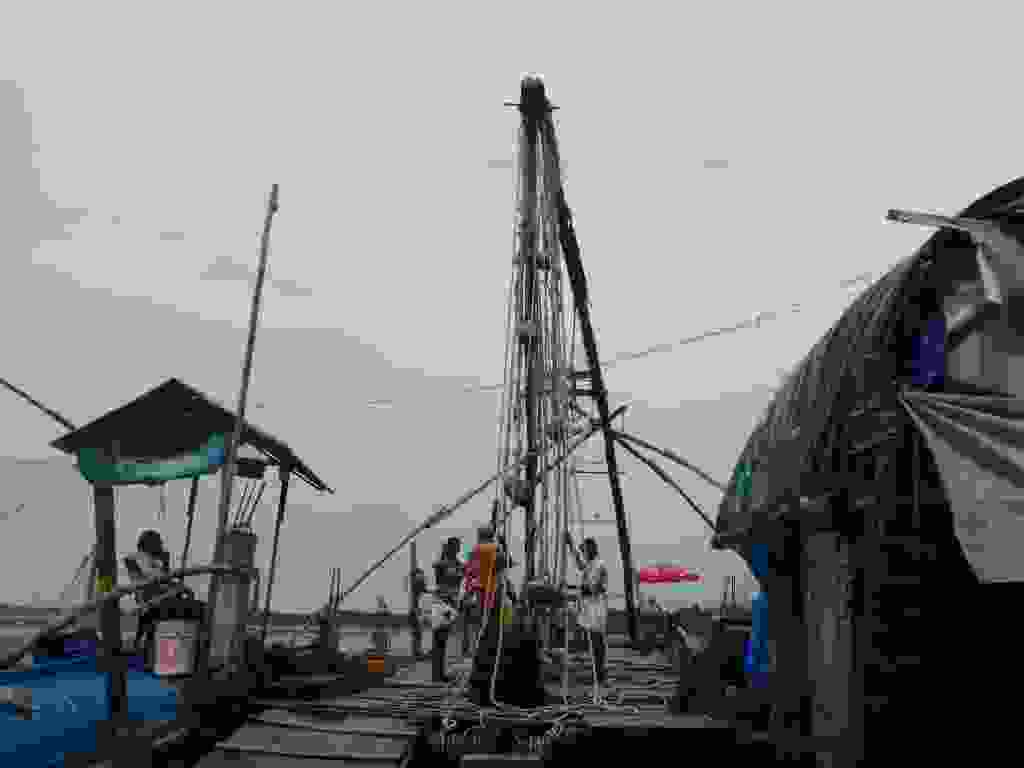
\includegraphics[width=\mywidth]{../wp-content/uploads/2015/11/wpid-oi000181-1024x768.jpg} } 
 \newline
 \newline
\centerline{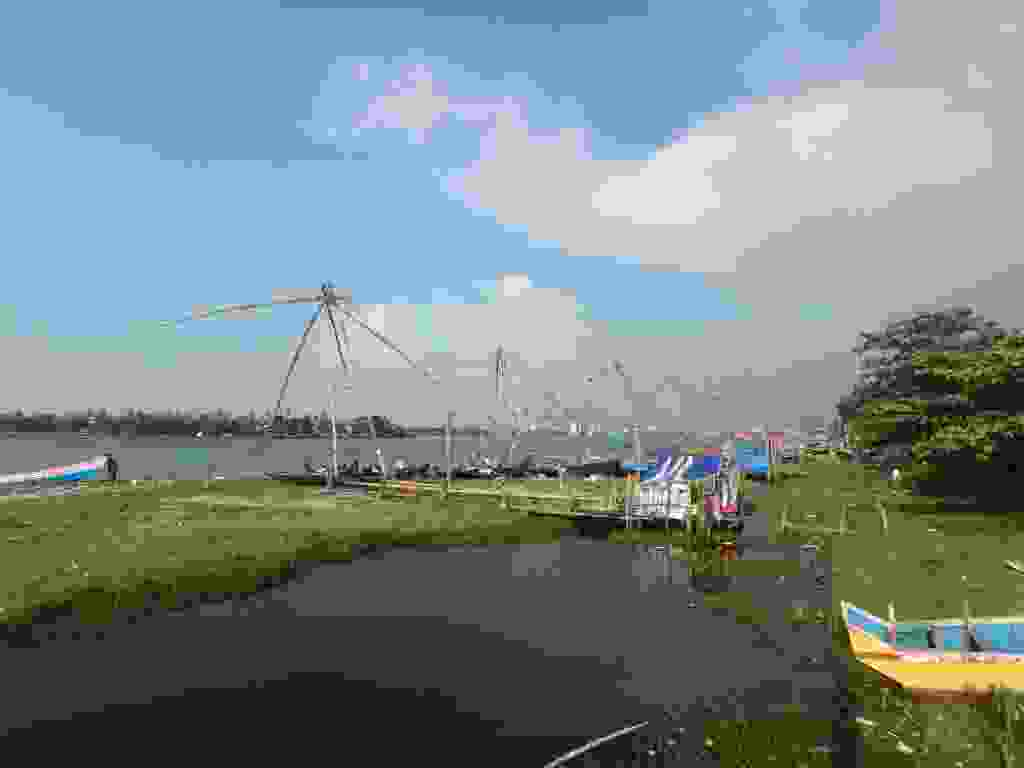
\includegraphics[width=\mywidth]{../wp-content/uploads/2015/11/wpid-oi000218-1024x768.jpg} } 
 \newline
 Le palais hollandais, de belles peintures murales à l'intérieur mais photos interdites \newline
 \newline
\centerline{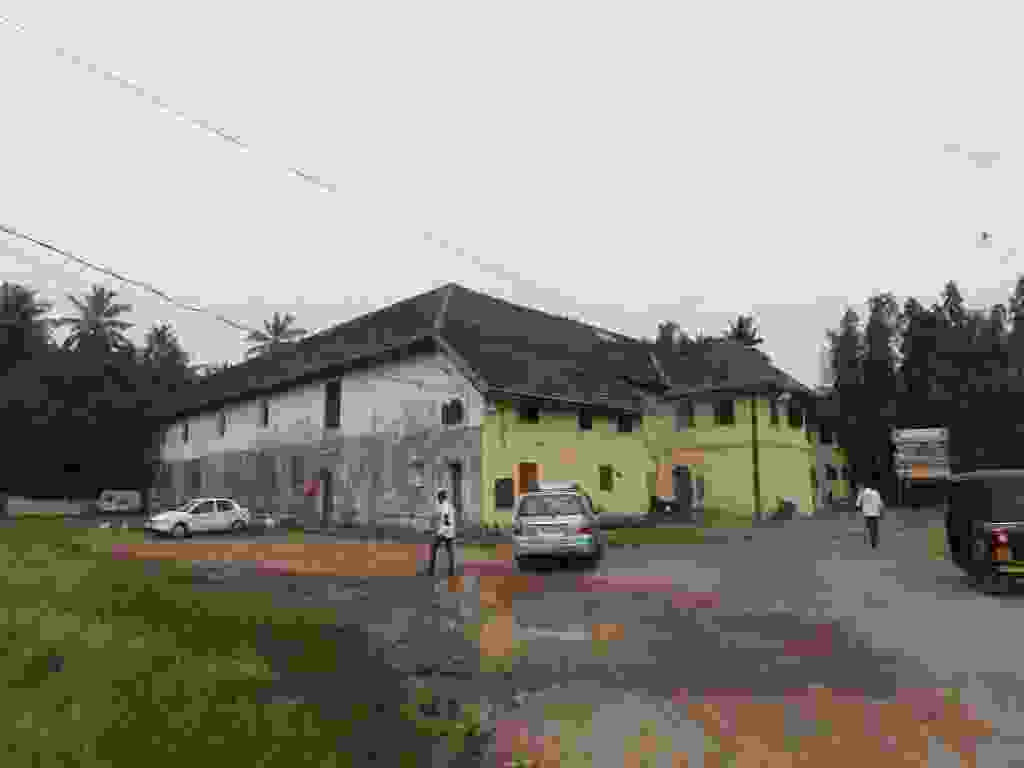
\includegraphics[width=\mywidth]{../wp-content/uploads/2015/11/wpid-oi000194-1024x768.jpg} } 
 \newline
 Église St Francis où Vasco de Gama a été enterré \newline
 \newline
\centerline{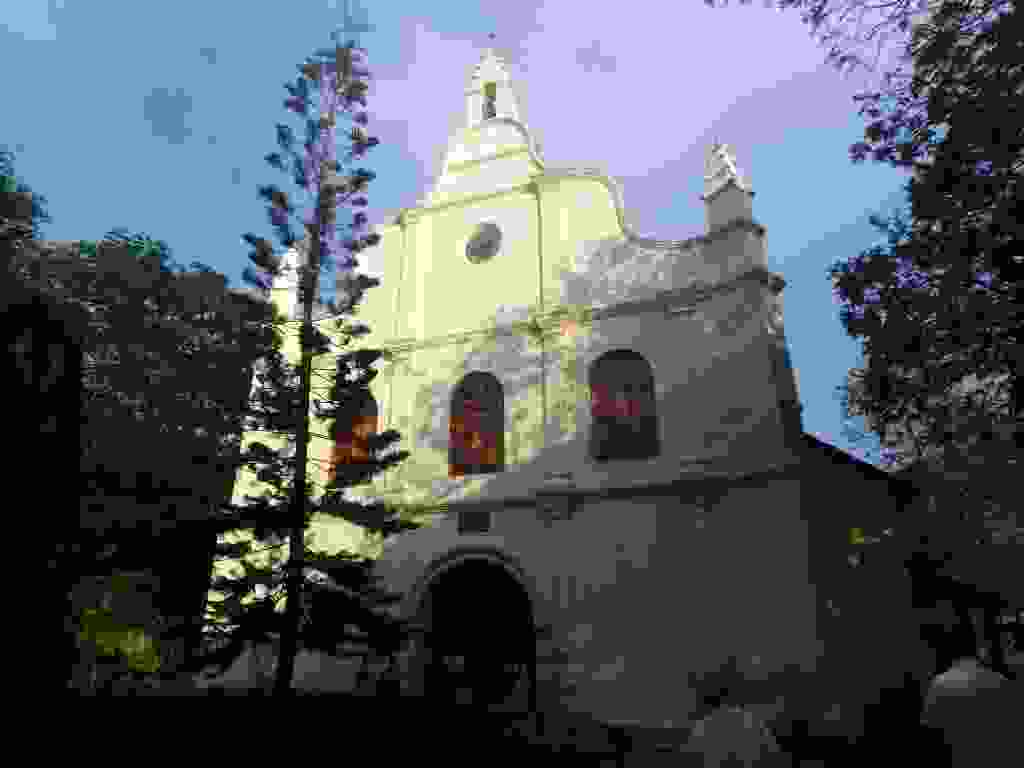
\includegraphics[width=\mywidth]{../wp-content/uploads/2015/11/wpid-oi000215-1024x768.jpg} } 
 \newline
 Quartier juif avec une très ancienne synagogue et des rues commerçantes \newline
 \newline
\centerline{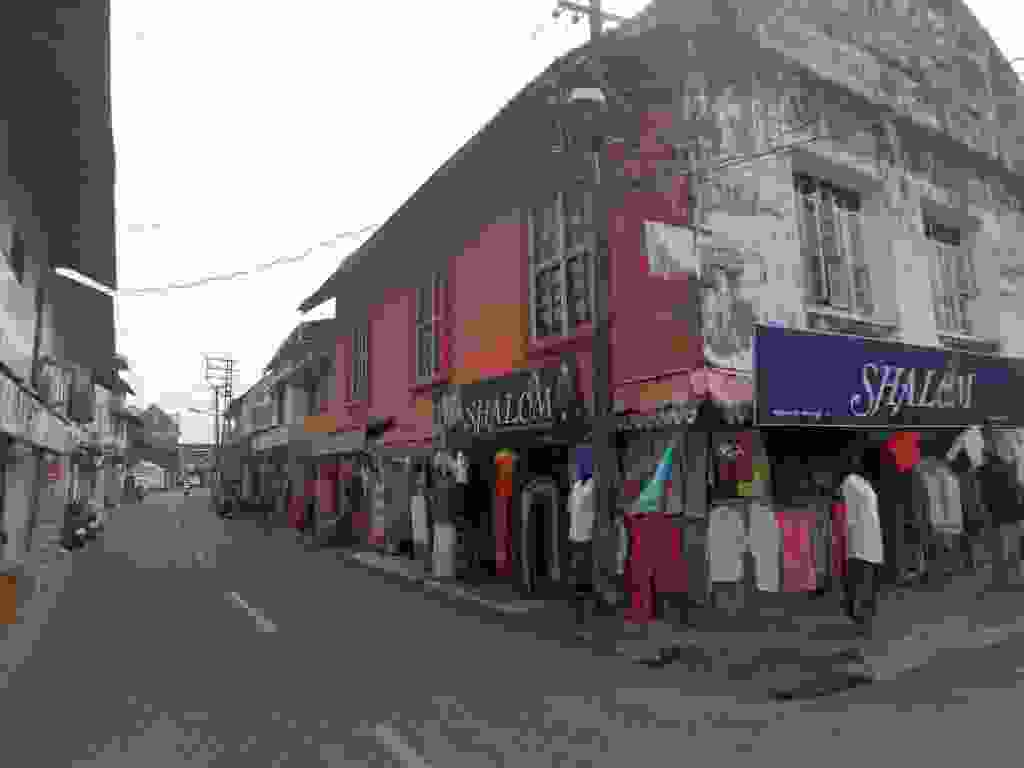
\includegraphics[width=\mywidth]{../wp-content/uploads/2015/11/wpid-oi000197-1024x768.jpg} } 
 \newline
 \newline
\centerline{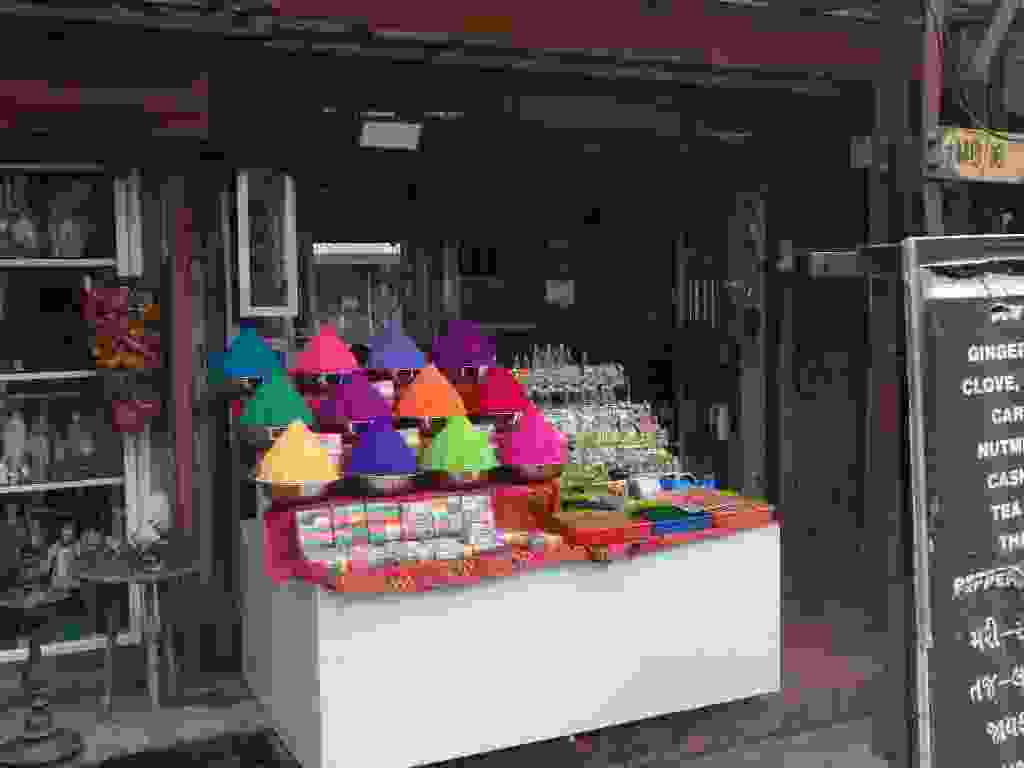
\includegraphics[width=\mywidth]{../wp-content/uploads/2015/11/wpid-oi000196-1024x768.jpg} } 
 \newline
 Les rickshaws qui proposent des tours gratuits à condition d'entrer dans une boutique de souvenirs \newline
 \newline
\centerline{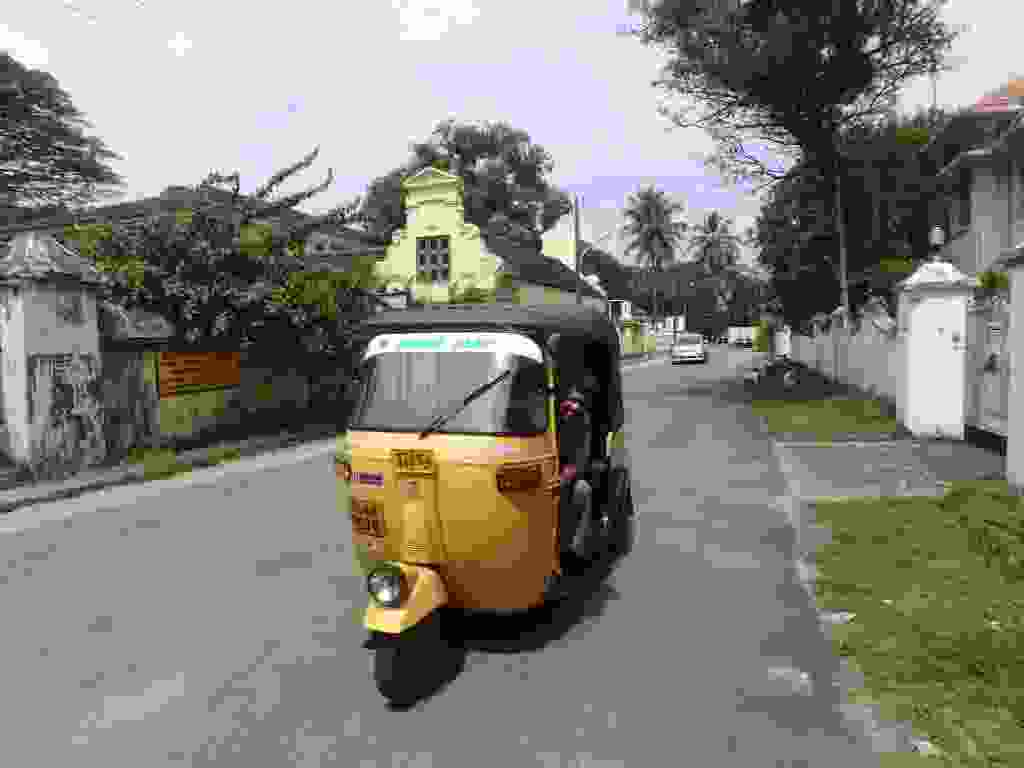
\includegraphics[width=\mywidth]{../wp-content/uploads/2015/11/wpid-oi000186-1024x768.jpg} } 
 \newline
 Je rejoins ensuite un groupe de «vacanciers» toulousains, l'occasion de faire du yoga dans un cadre agréable \newline
 \newline
\centerline{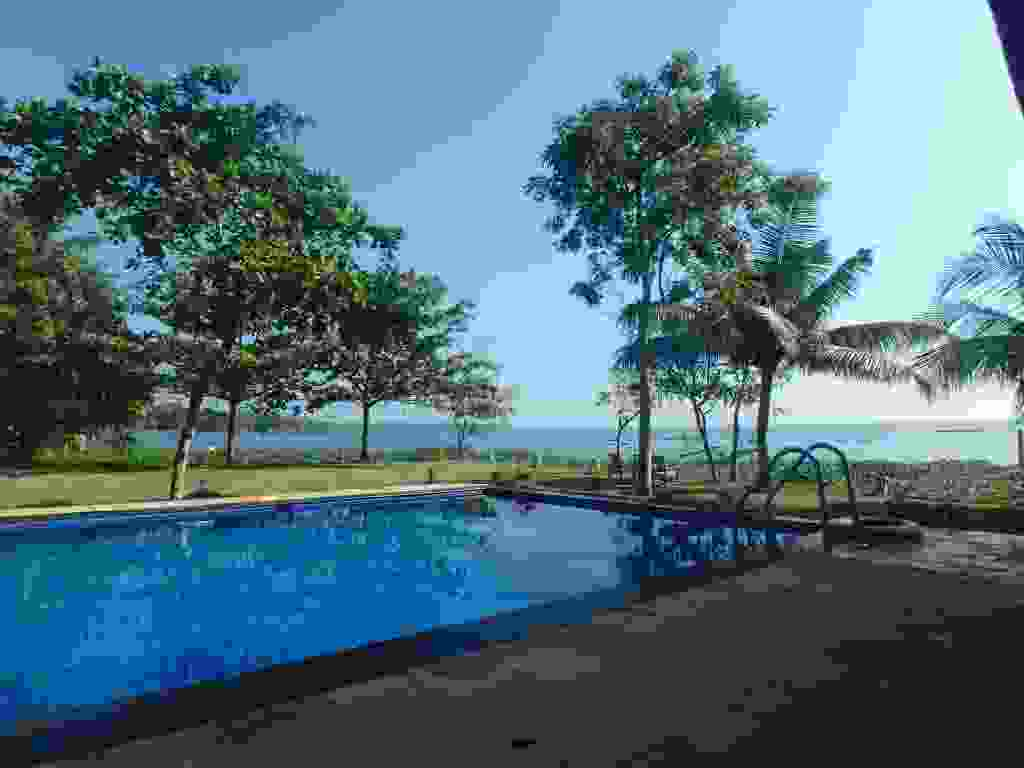
\includegraphics[width=\mywidth]{../wp-content/uploads/2015/11/wpid-oi000210-1024x768.jpg} } 
 \newline
 \newline
\centerline{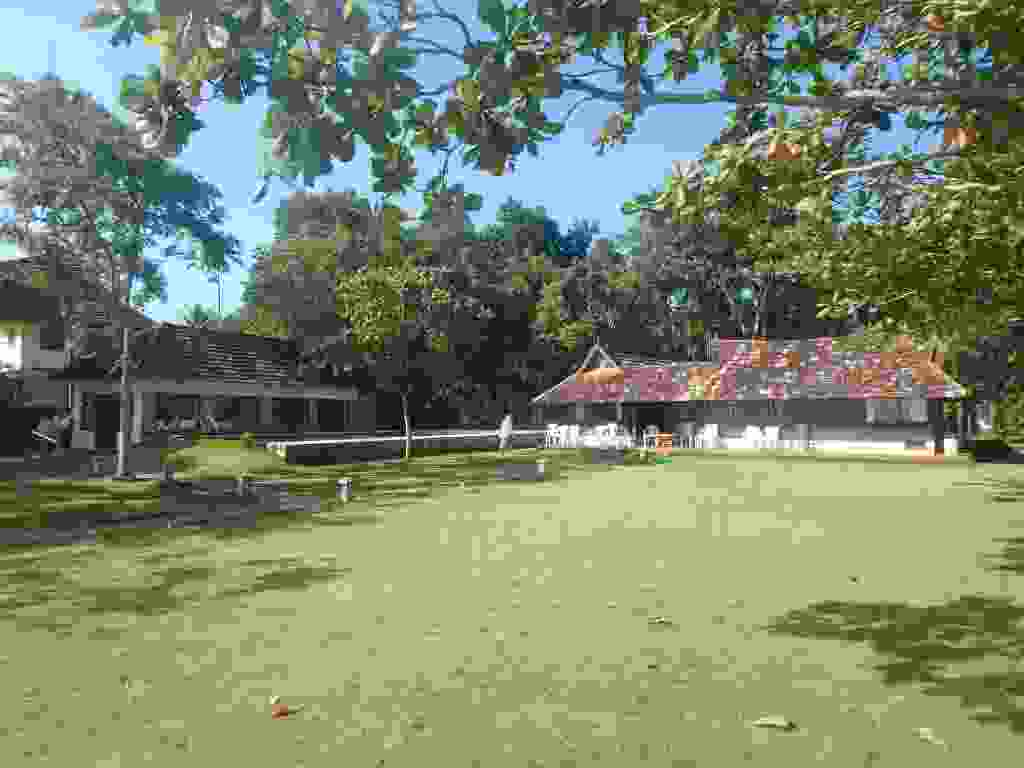
\includegraphics[width=\mywidth]{../wp-content/uploads/2015/11/wpid-oi000212-1024x768.jpg} } 
 \newline
 Et une excursion en bateau dans les backwaters \newline
 \newline
\centerline{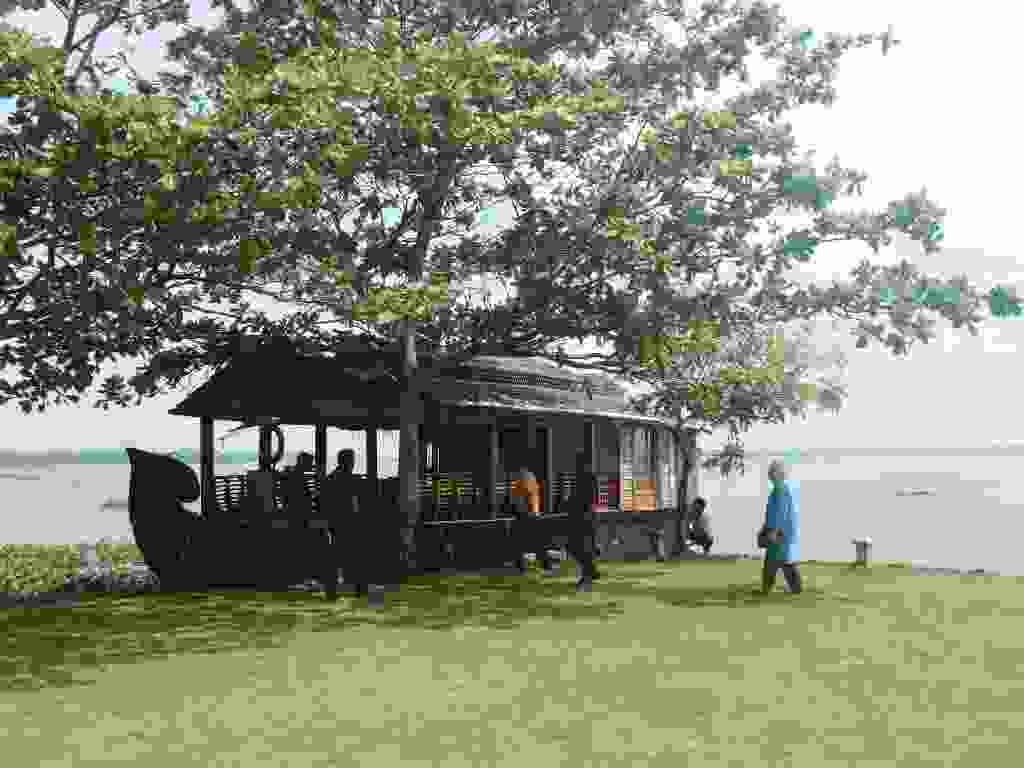
\includegraphics[width=\mywidth]{../wp-content/uploads/2015/11/wpid-oi000221-1024x768.jpg} } 
 \newline
 \newline
\centerline{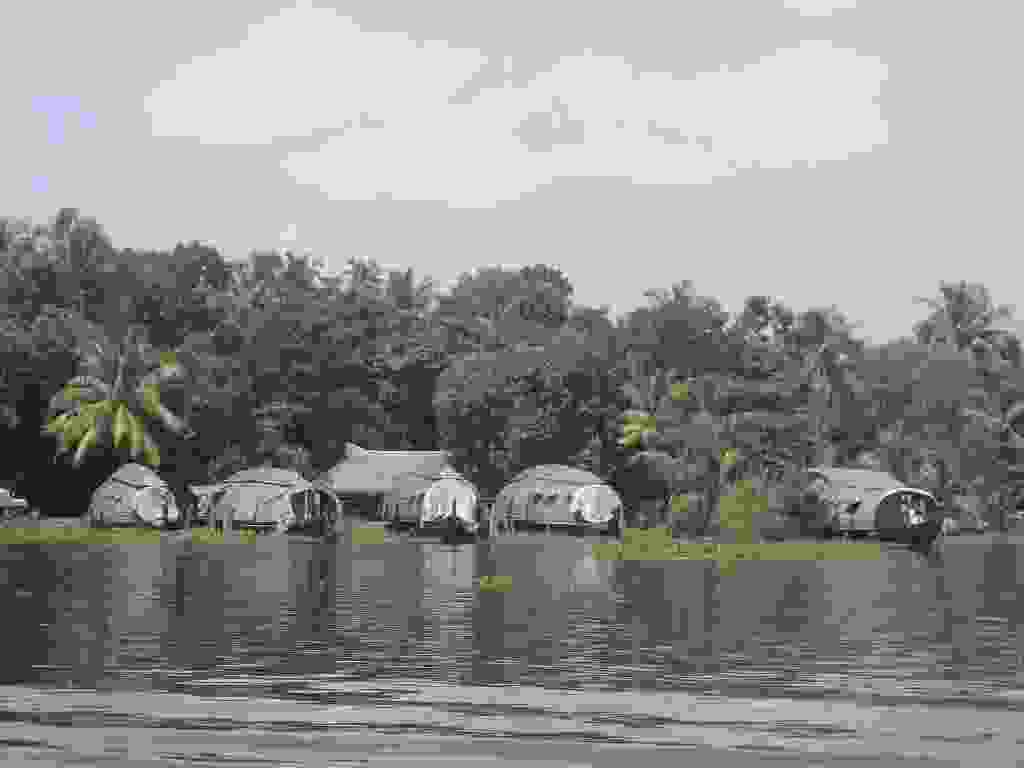
\includegraphics[width=\mywidth]{../wp-content/uploads/2015/11/wpid-oi000226-1024x768.jpg} } 
 \newline
 \newline
\centerline{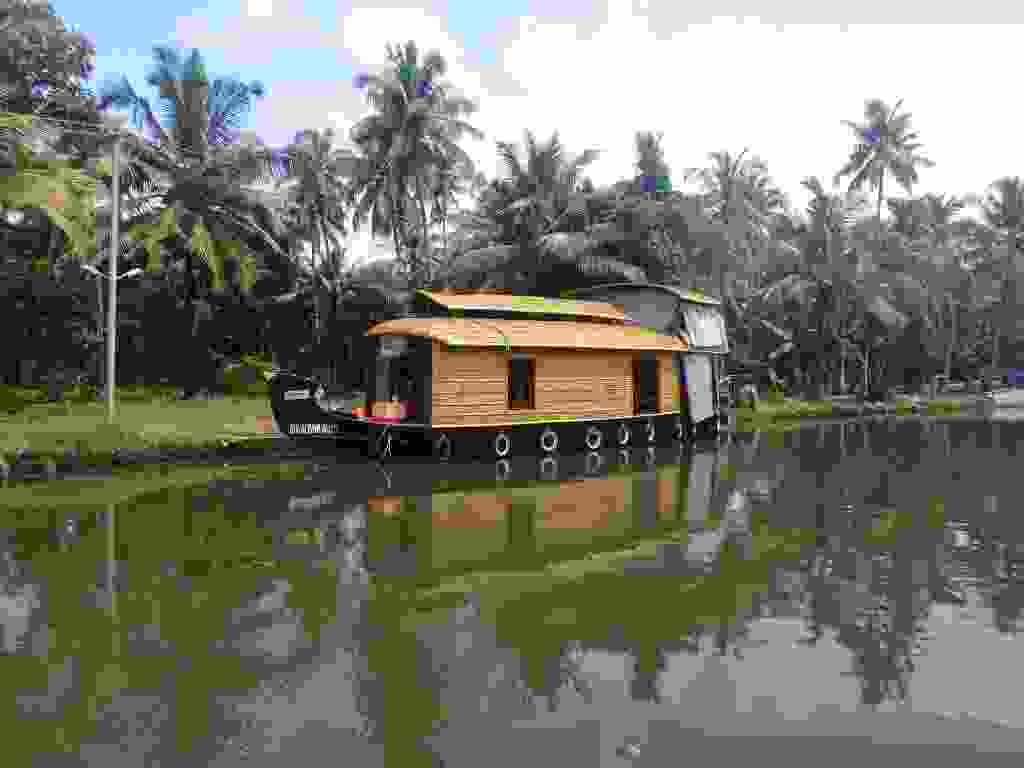
\includegraphics[width=\mywidth]{../wp-content/uploads/2015/11/wpid-oi000234-1024x768.jpg} } 
 \newline
 \newline
\centerline{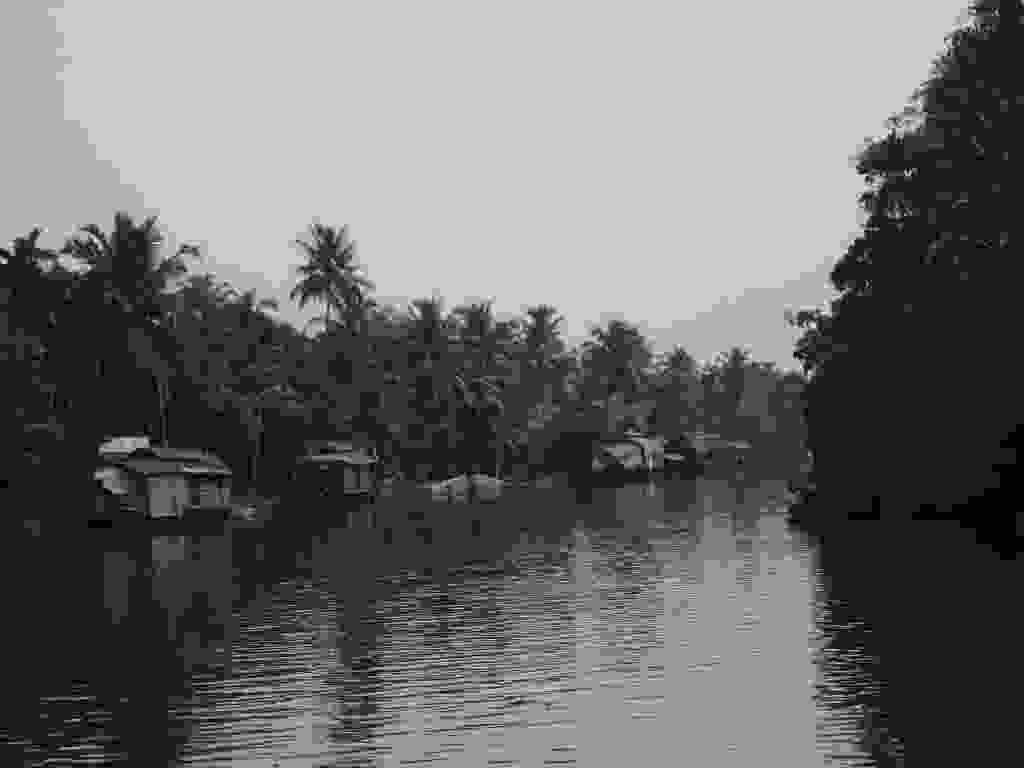
\includegraphics[width=\mywidth]{../wp-content/uploads/2015/11/wpid-oi000233-1024x768.jpg} } 
 \newline
 \newline
\centerline{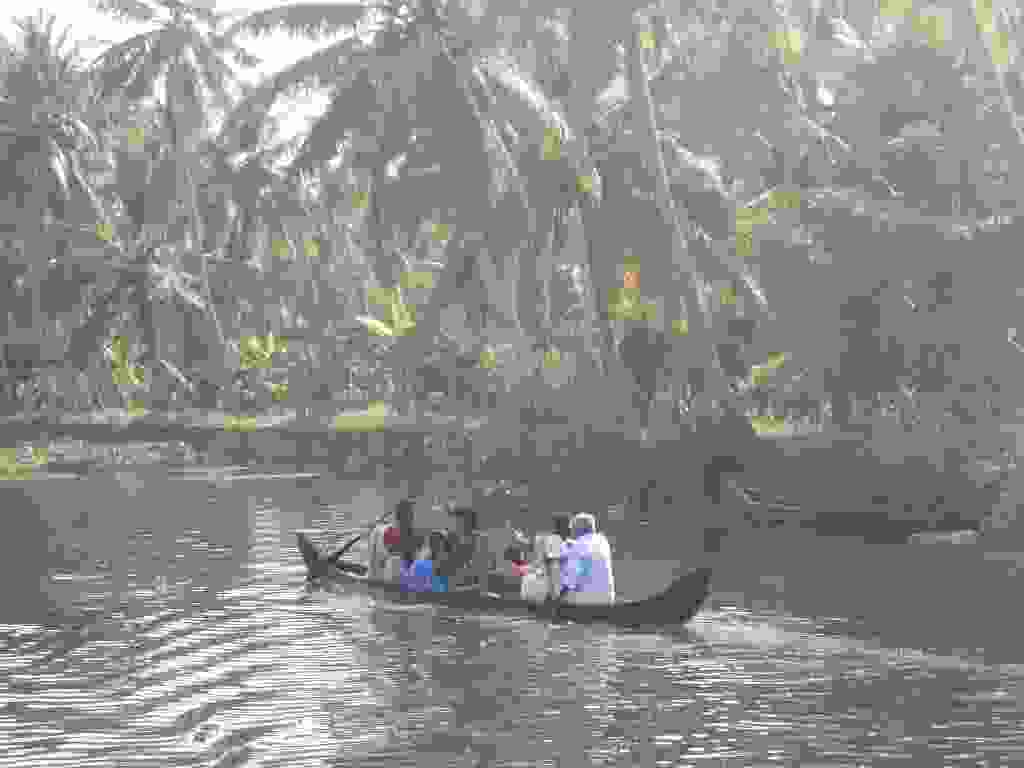
\includegraphics[width=\mywidth]{../wp-content/uploads/2015/11/wpid-oi000245-1024x768.jpg} } 
 \newline
 \newline
\centerline{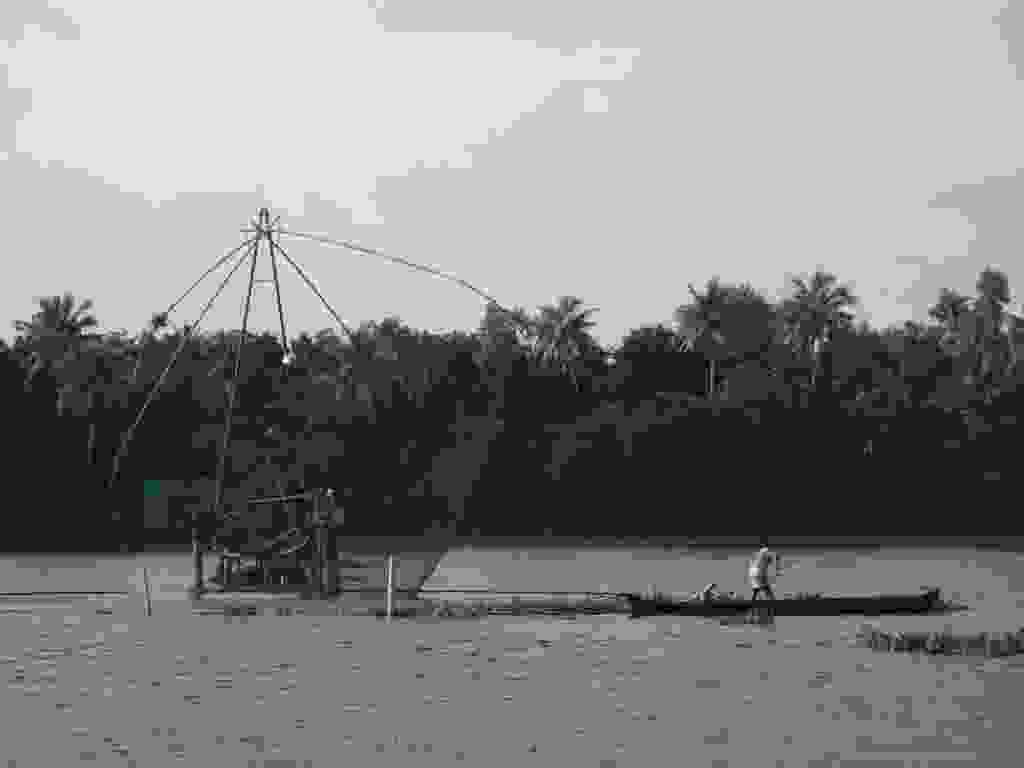
\includegraphics[width=\mywidth]{../wp-content/uploads/2015/11/wpid-oi000250-1024x768.jpg} } 
 \newline
 Des femmes font la lessive en frappant le linge sur une pierre \newline
 \newline
\centerline{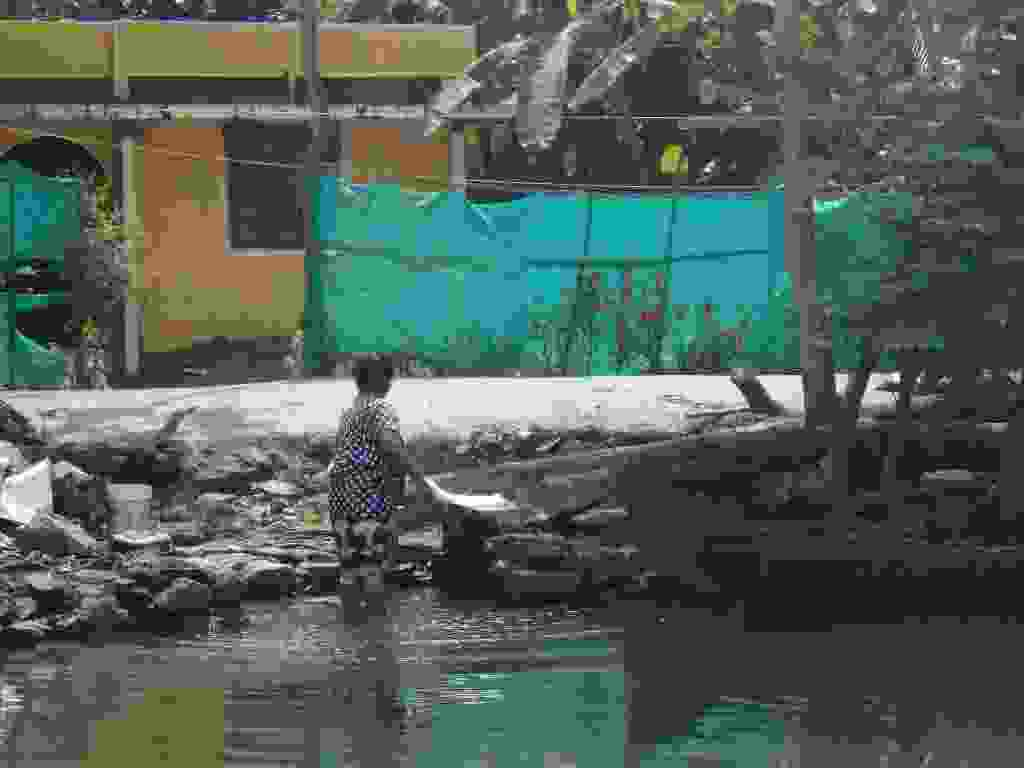
\includegraphics[width=\mywidth]{../wp-content/uploads/2015/11/wpid-oi000239-1024x768.jpg} } 
 \newline
 \newline
\centerline{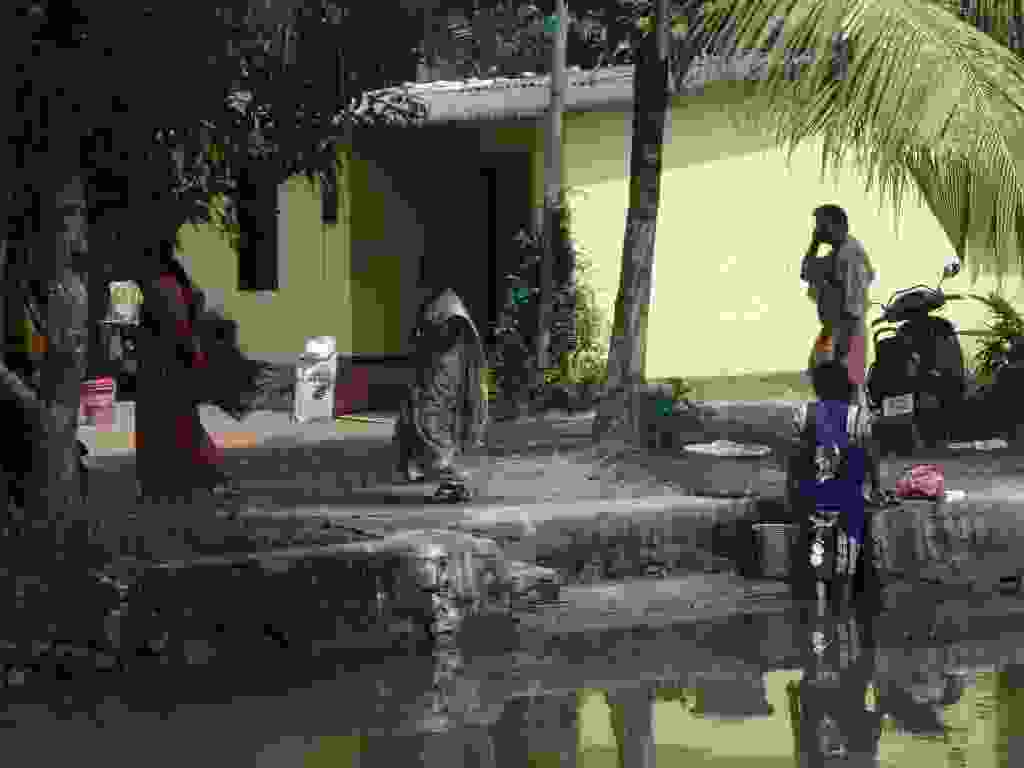
\includegraphics[width=\mywidth]{../wp-content/uploads/2015/11/wpid-oi000235-1024x768.jpg} } 
 \newline
 En descendant du bateau pour se balader on croise un gros lézard \newline
 \newline
\centerline{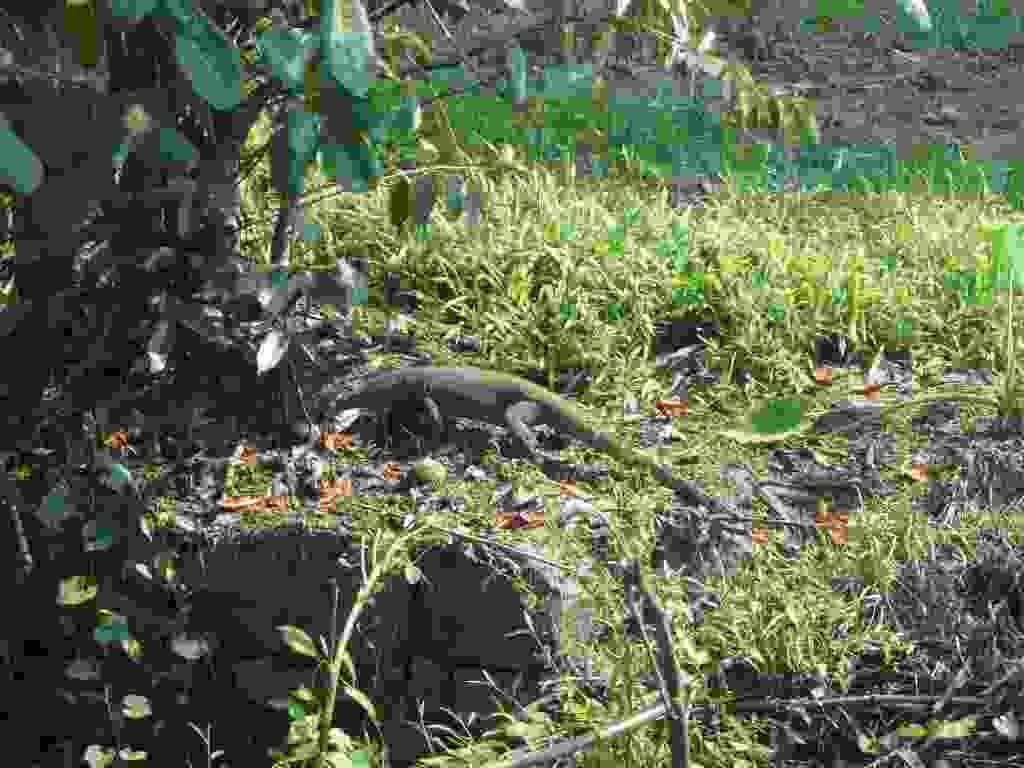
\includegraphics[width=\mywidth]{../wp-content/uploads/2015/11/wpid-oi000244-1024x768.jpg} } 
 \newline
 Je repars en vélo vers l'intérieur des terres, les gens sont amicaux : énormément de saluts à mon passage et souvent des motos viennent rouler à côté de moi pour discuter \newline
 Beaucoup de grandes maisons souvent bien colorées \newline
 \newline
\centerline{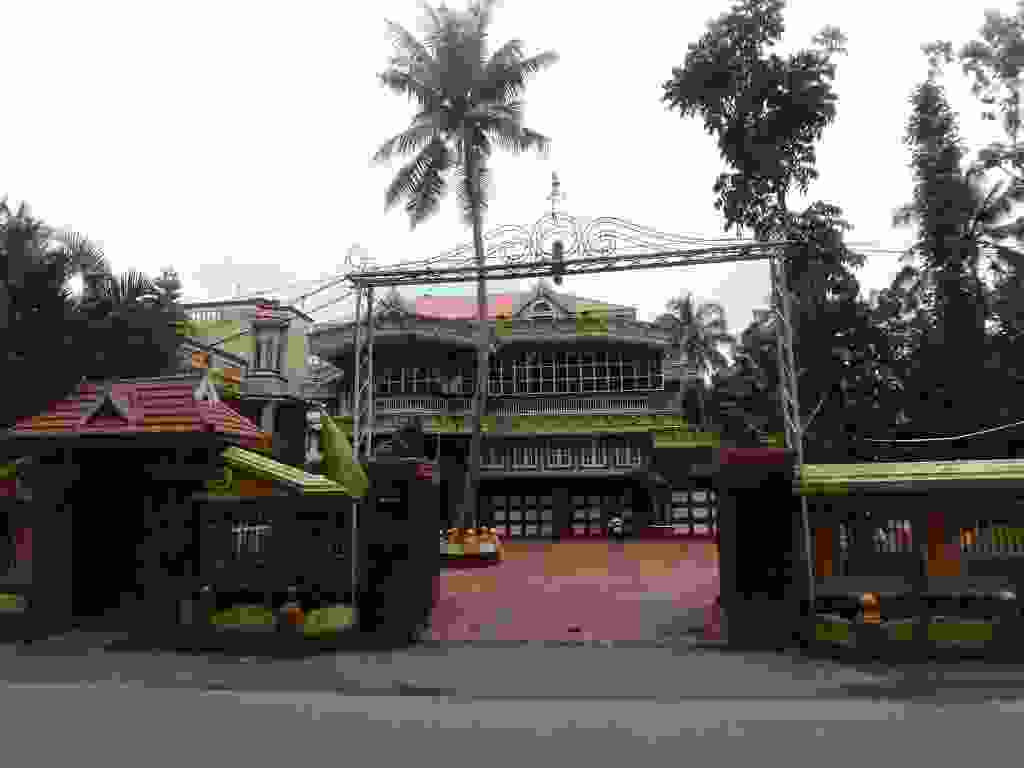
\includegraphics[width=\mywidth]{../wp-content/uploads/2015/11/wpid-oi000260-1024x768.jpg} } 
 \newline
 Encore un pays avec une belle variété de fruits \newline
 \newline
\centerline{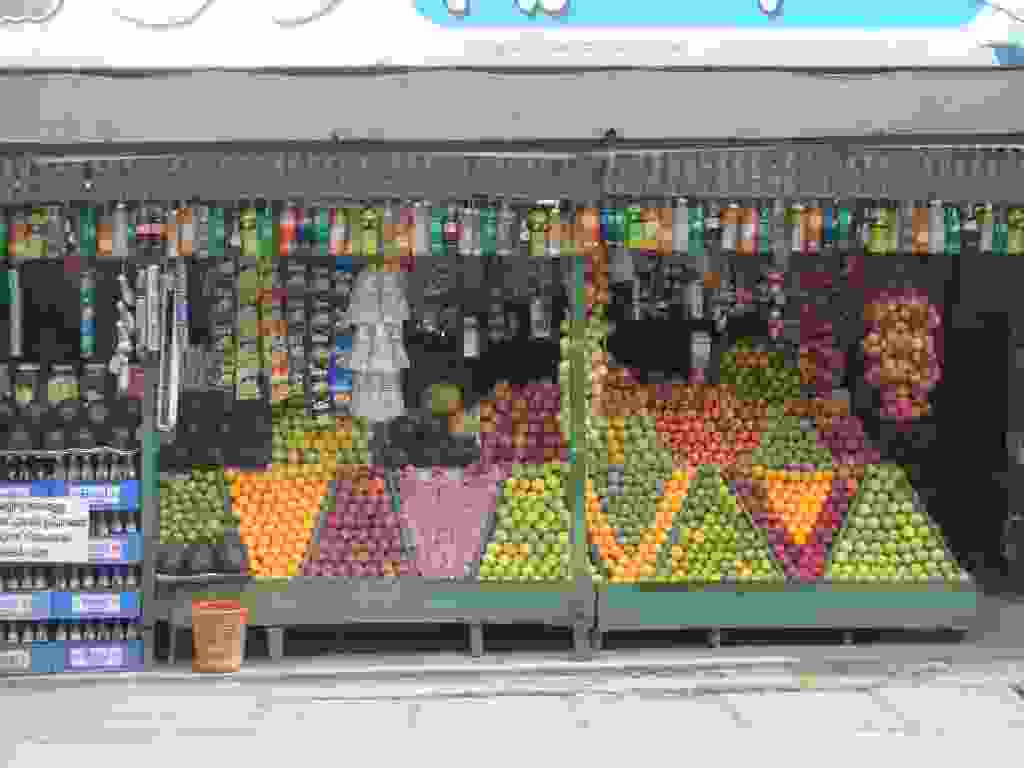
\includegraphics[width=\mywidth]{../wp-content/uploads/2015/11/wpid-oi000262-1024x768.jpg} } 
 \newline
 A côté des cultures d'ananas, le verre de jus frais à 35 centimes ! \newline
 \newline
\centerline{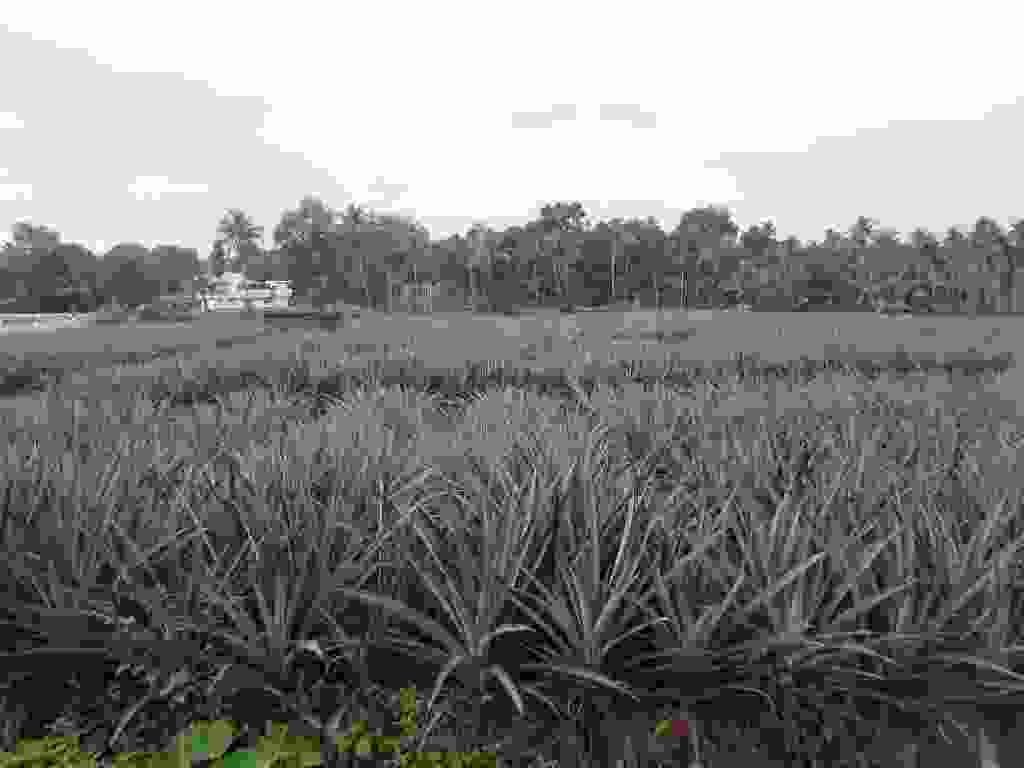
\includegraphics[width=\mywidth]{../wp-content/uploads/2015/11/wpid-oi000264-1024x768.jpg} } 
 \newline
 \newline
\centerline{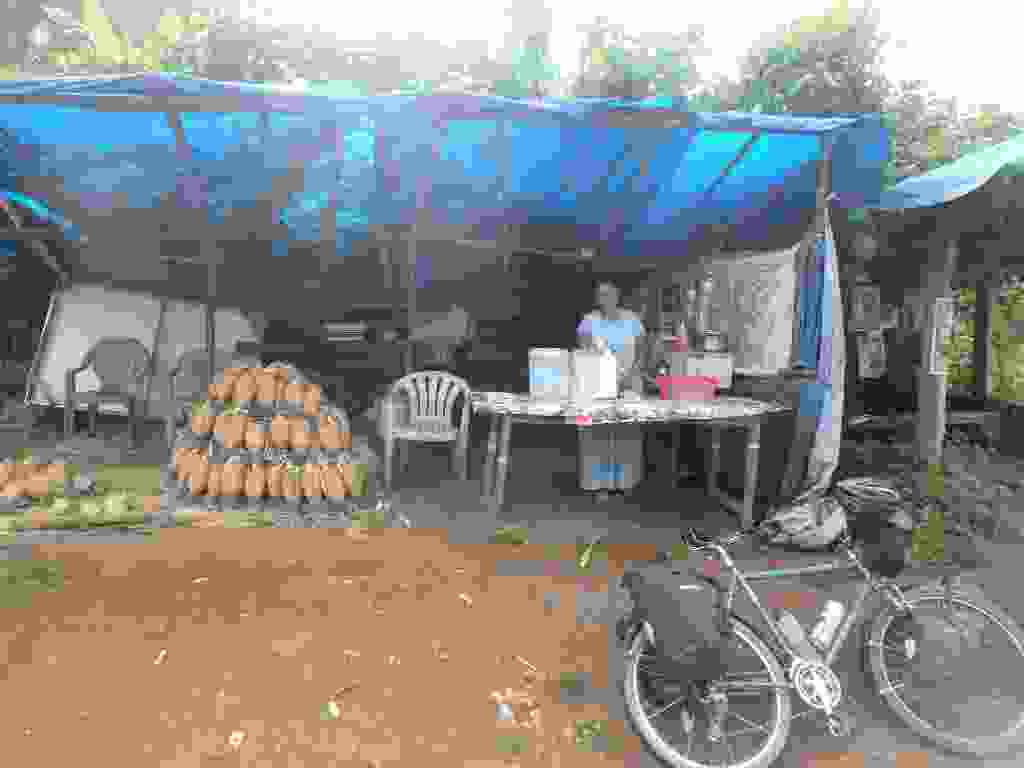
\includegraphics[width=\mywidth]{../wp-content/uploads/2015/11/wpid-oi000263-1024x768.jpg} } 
 \newline
 Je passe devant une répétition de percussions, le prof me fait signe de venir voir \newline
 \newline
\centerline{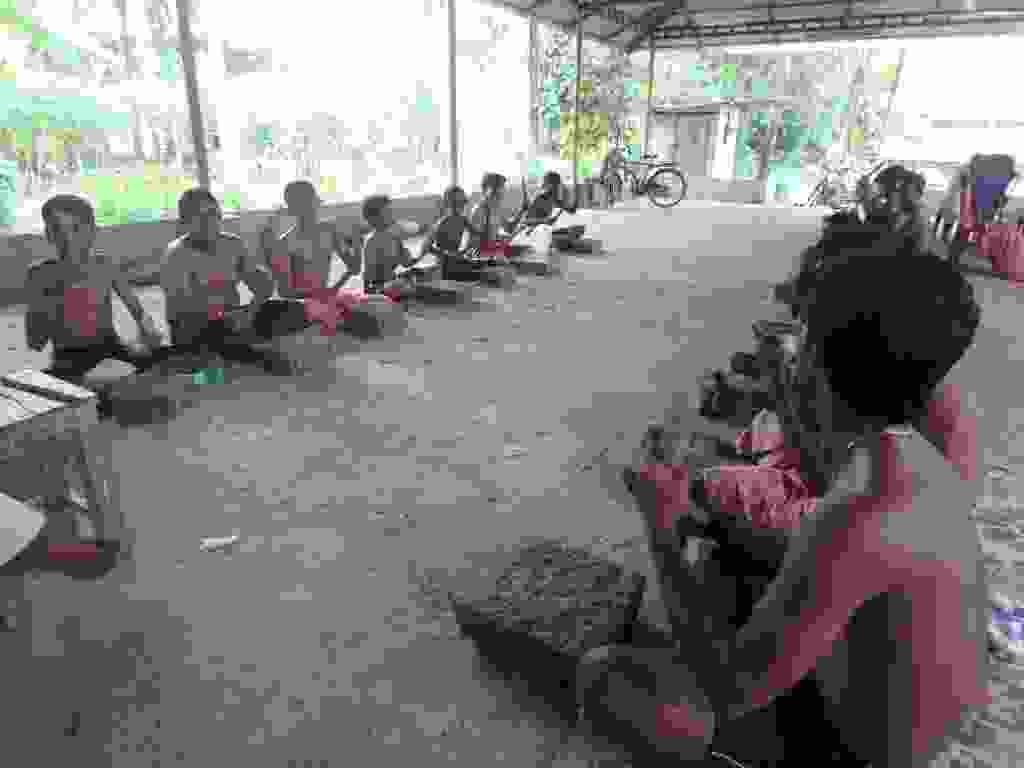
\includegraphics[width=\mywidth]{../wp-content/uploads/2015/11/wpid-oi000266-1024x768.jpg} } 
 \newline
 \newline
\centerline{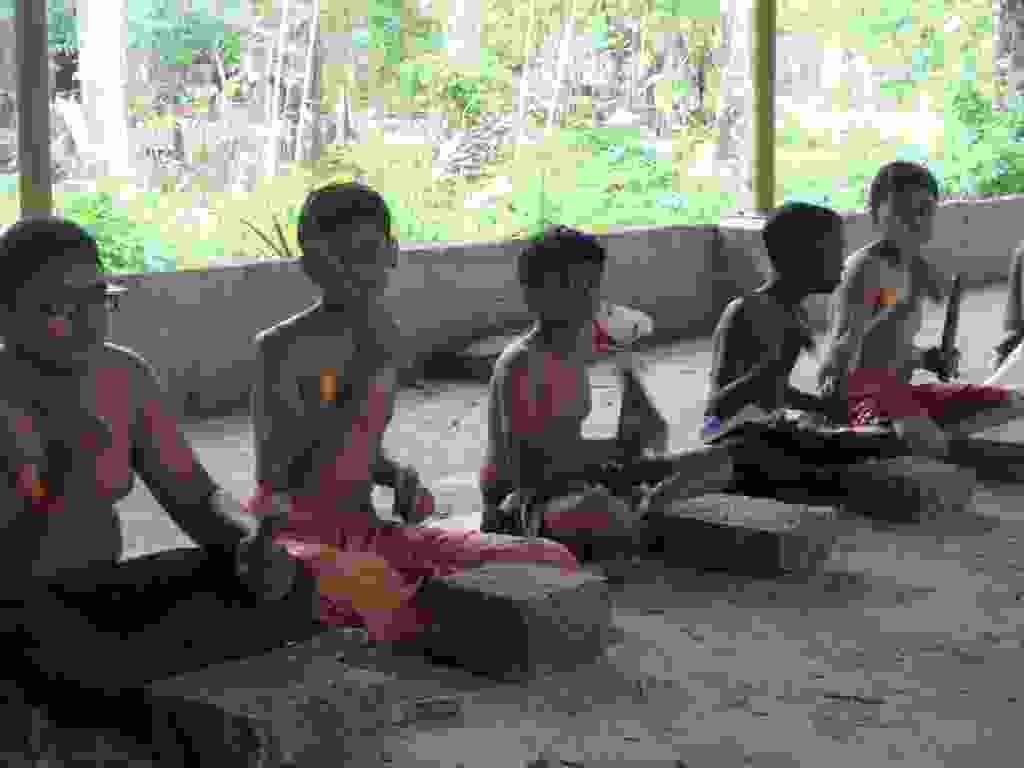
\includegraphics[width=\mywidth]{../wp-content/uploads/2015/11/wpid-oi000267-1024x768.jpg} } 
 \newline
 \newline
\centerline{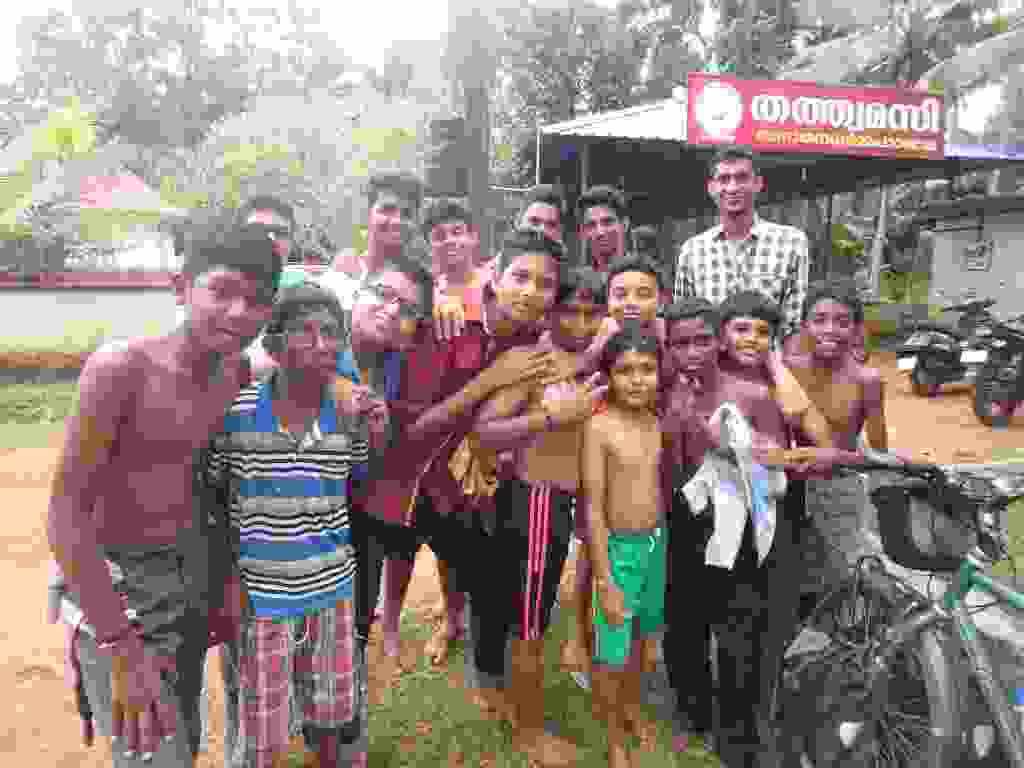
\includegraphics[width=\mywidth]{../wp-content/uploads/2015/11/wpid-oi000269-1024x768.jpg} } 
 \newline
 Arrêt pour visiter un jardin de plantes ayurvédiques \newline
 \newline
\centerline{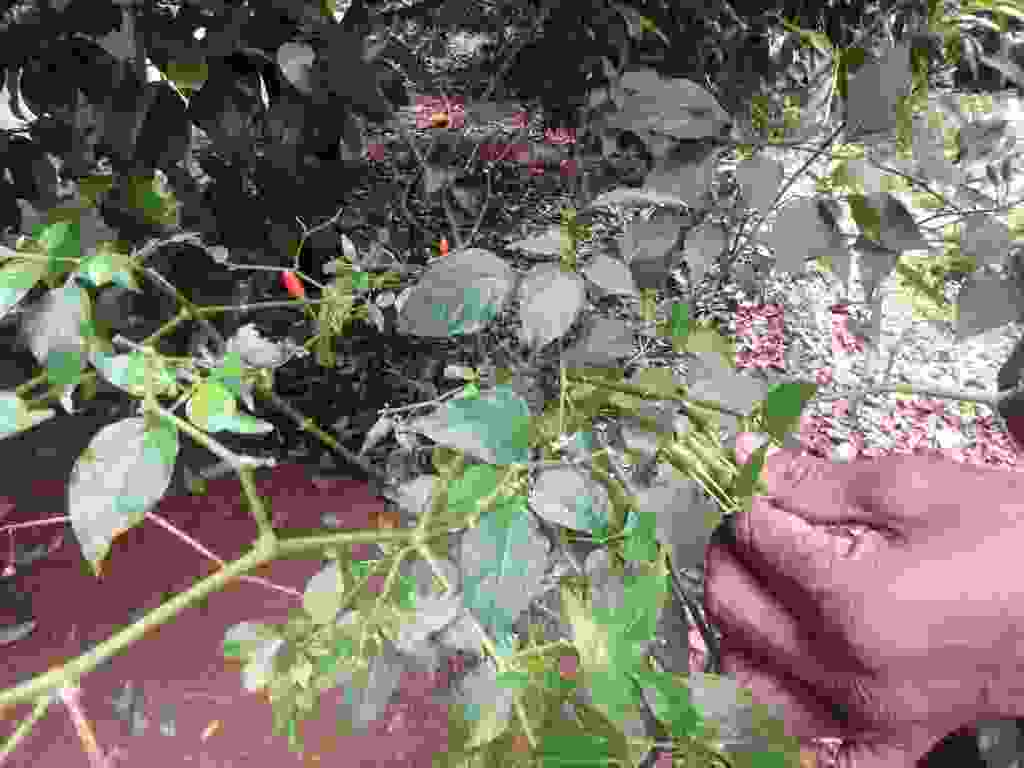
\includegraphics[width=\mywidth]{../wp-content/uploads/2015/11/wpid-oi000280-1024x768.jpg} } 
 \newline
 \newline
\centerline{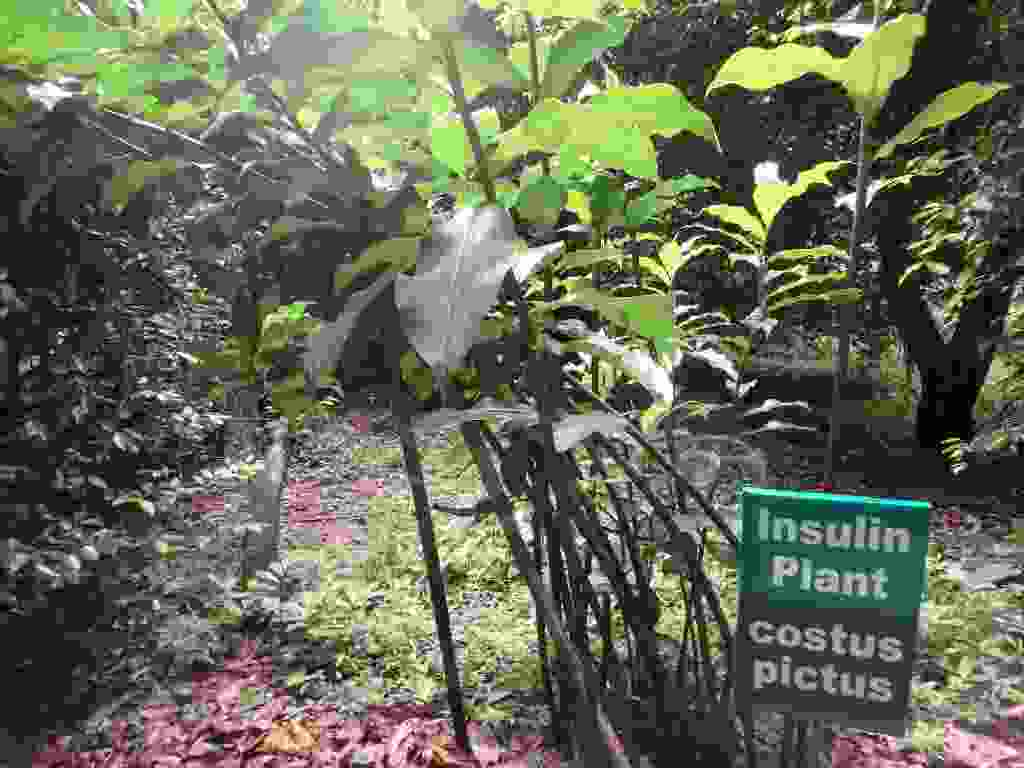
\includegraphics[width=\mywidth]{../wp-content/uploads/2015/11/wpid-oi000289-1024x768.jpg} } 
 \newline
 La route s'élève en s'approchant de Munnar \newline
 \newline
\centerline{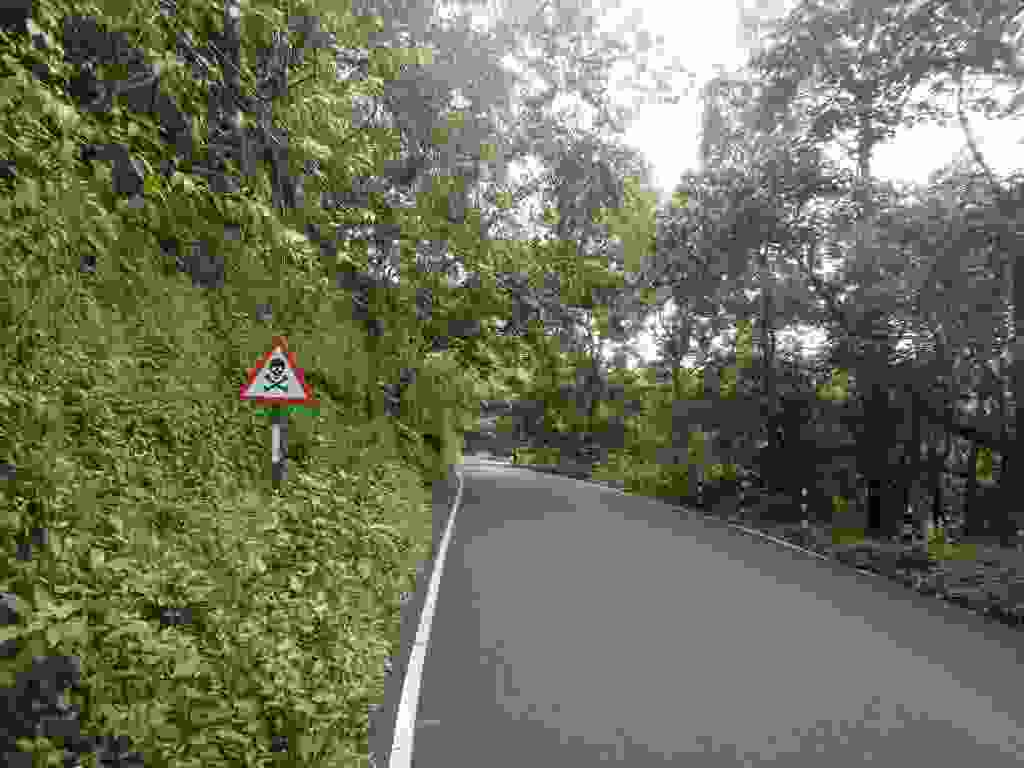
\includegraphics[width=\mywidth]{../wp-content/uploads/2015/11/wpid-oi000272-1024x768.jpg} } 
 \newline
 \newline
\centerline{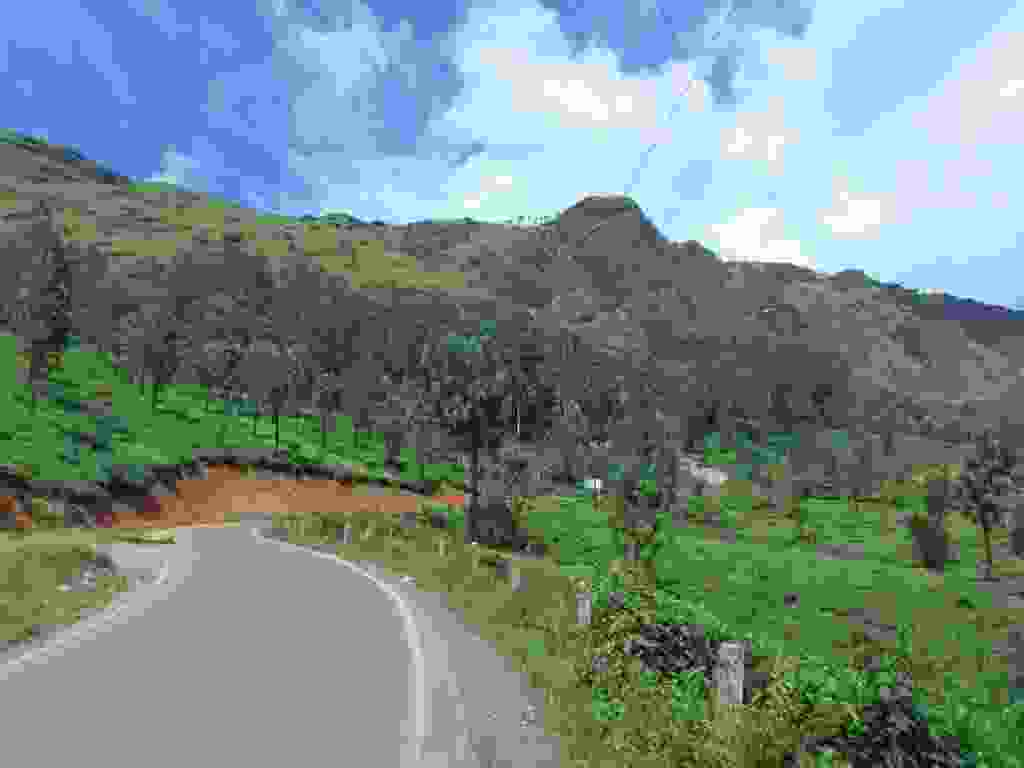
\includegraphics[width=\mywidth]{../wp-content/uploads/2015/11/wpid-oi00021801.jpg-1024x768.jpg} } 
 \newline
 Munnar à environ 1500m d'altitude, un peu de fraîcheur par rapport à la chaleur humide sur la côte \newline
 \newline
\centerline{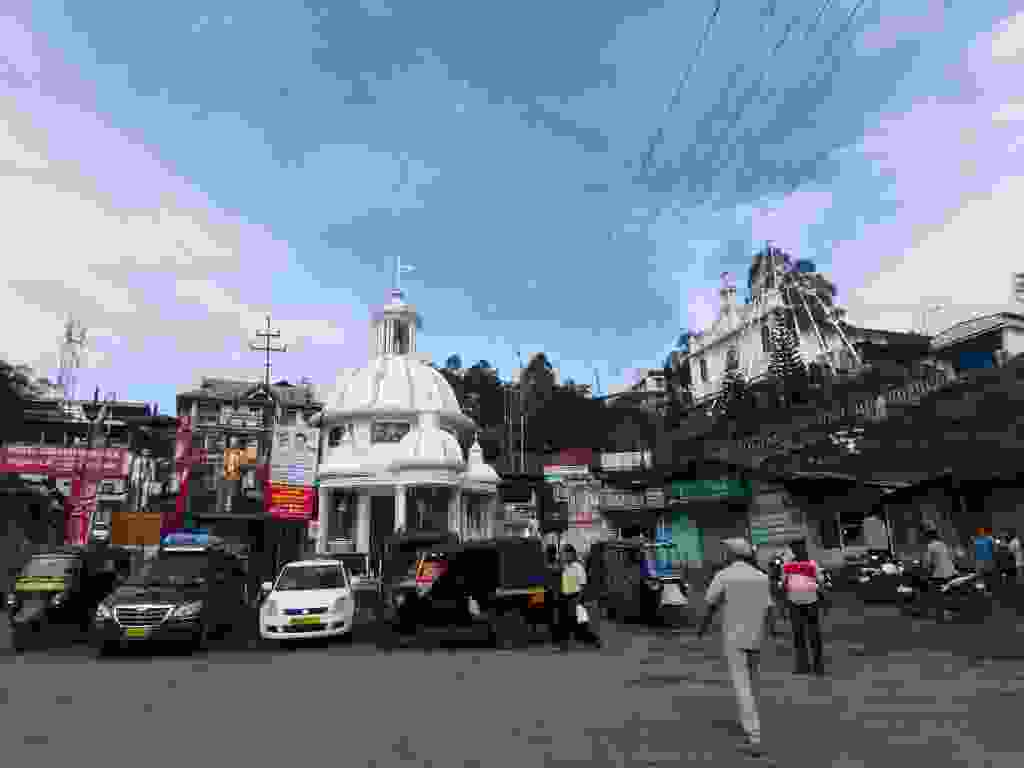
\includegraphics[width=\mywidth]{../wp-content/uploads/2015/11/wpid-oi000293-1024x768.jpg} } 
 \newline
 \newline
\centerline{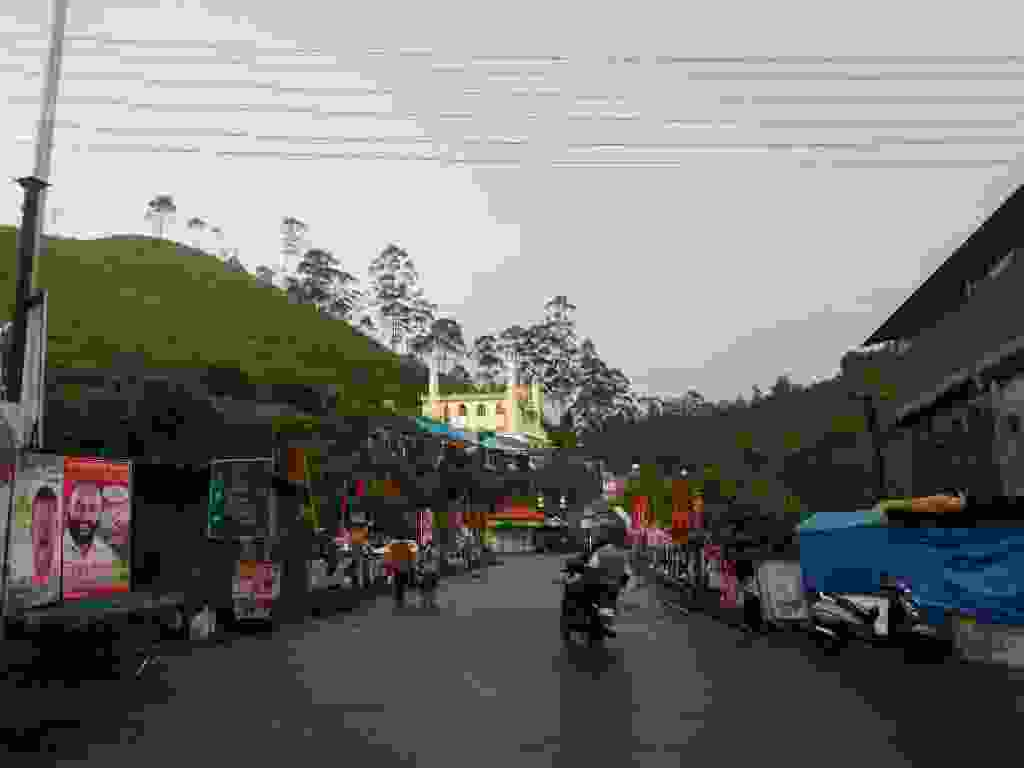
\includegraphics[width=\mywidth]{../wp-content/uploads/2015/11/wpid-oi000308-1024x768.jpg} } 
 \newline
 Les alentours sont couverts de plantations de thé \newline
 \newline
\centerline{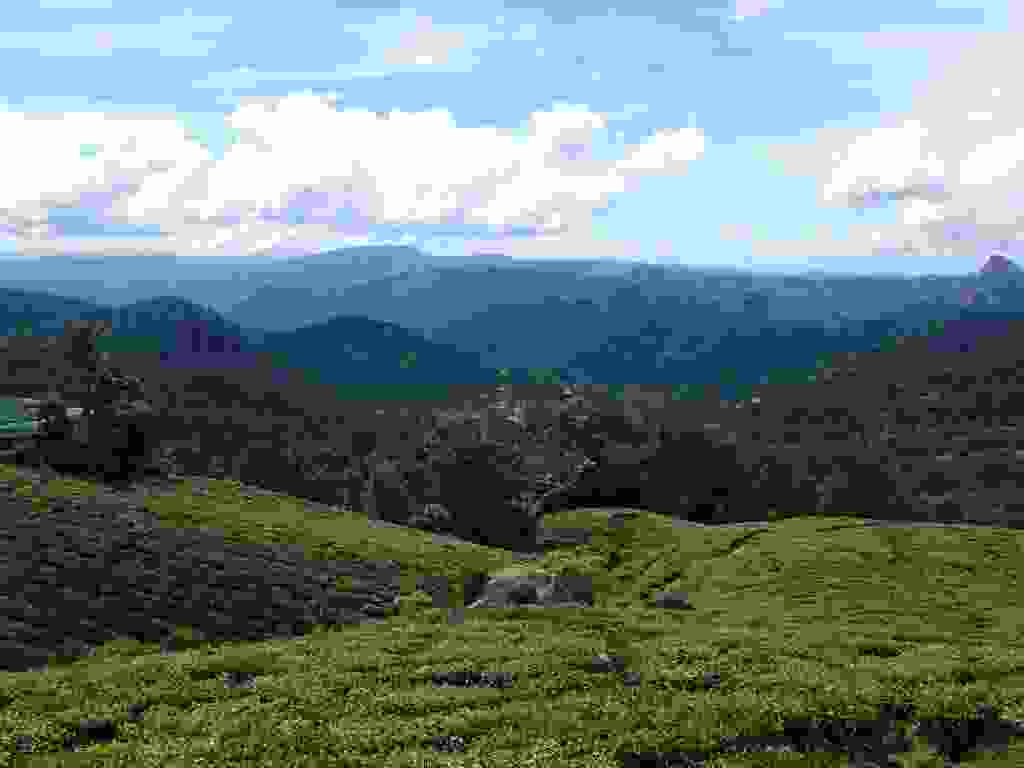
\includegraphics[width=\mywidth]{../wp-content/uploads/2015/11/wpid-oi00023301.jpg-1024x768.jpg} } 
 \newline
 \newline
\centerline{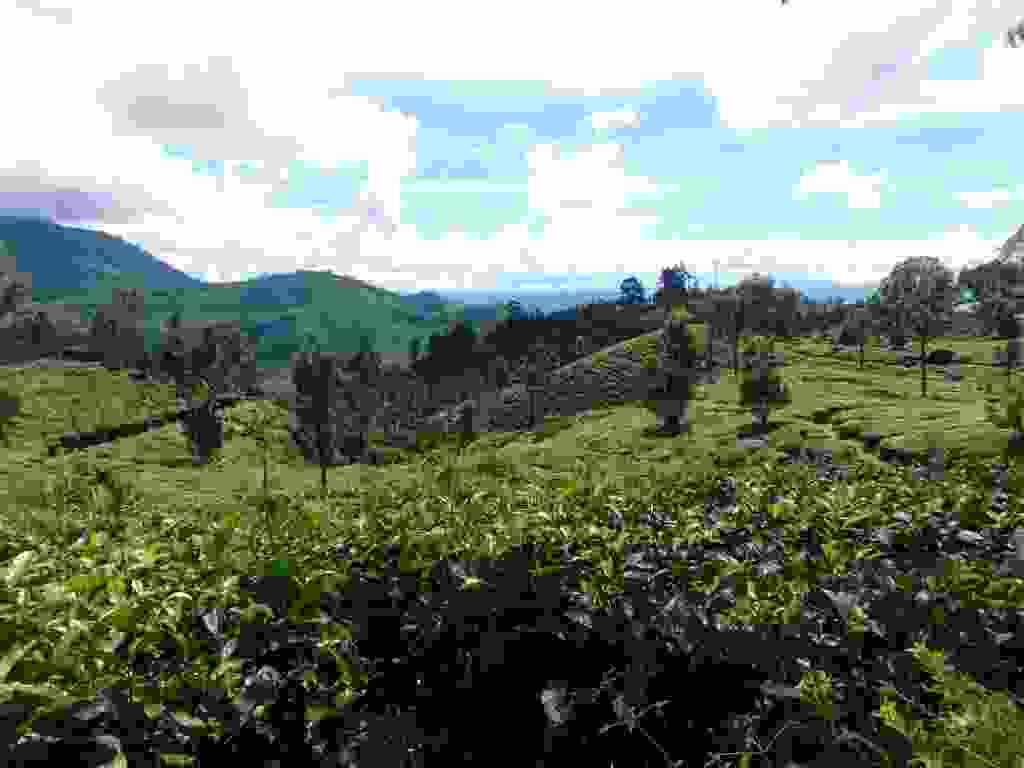
\includegraphics[width=\mywidth]{../wp-content/uploads/2015/11/wpid-oi00021501.jpg-1024x768.jpg} } 
 \newline
 Le musée du thé montre les machines pour fabriquer le thé noir \newline
 \newline
\centerline{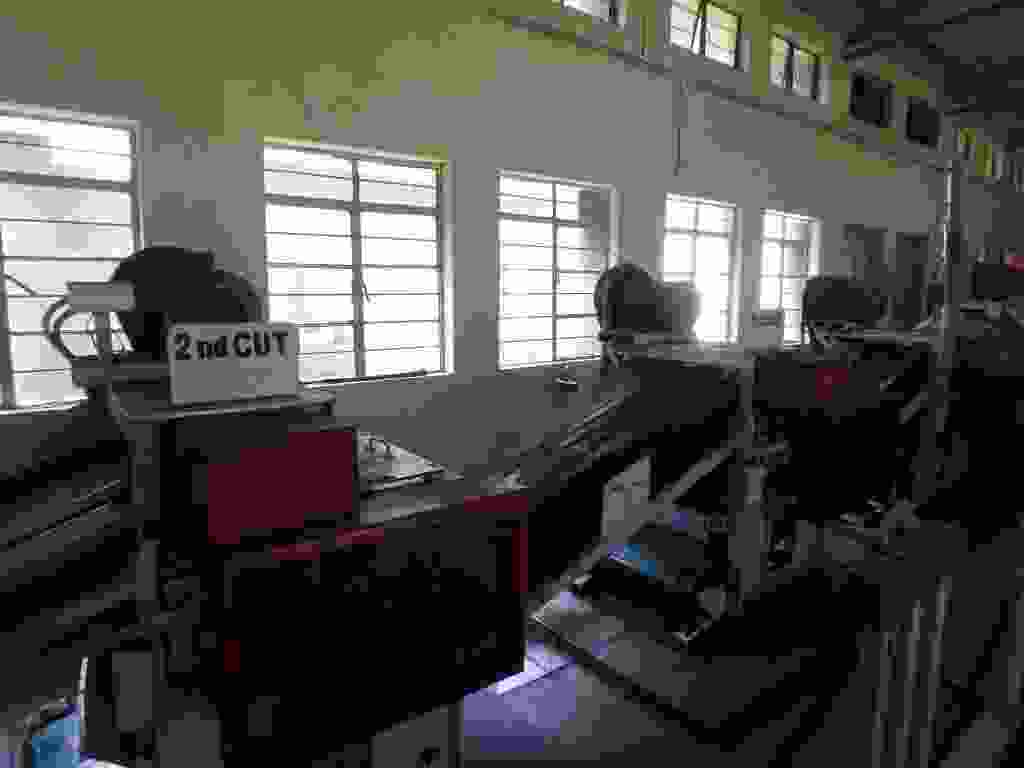
\includegraphics[width=\mywidth]{../wp-content/uploads/2015/11/wpid-oi00018601.jpg-1024x768.jpg} } 
 \newline
 Montée à la Top Station à plus de 2000m, jolie surprise au bord de la route \newline
 \newline
\centerline{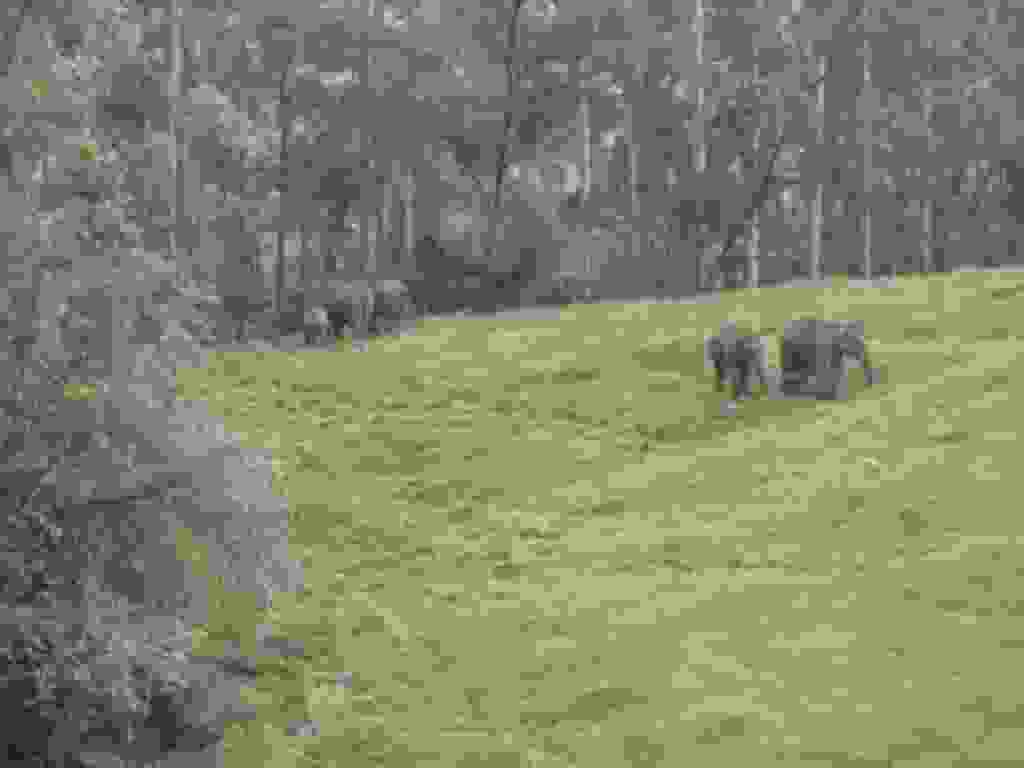
\includegraphics[width=\mywidth]{../wp-content/uploads/2015/11/wpid-oi000299-1024x768.jpg} } 
 \newline
 \newline
\centerline{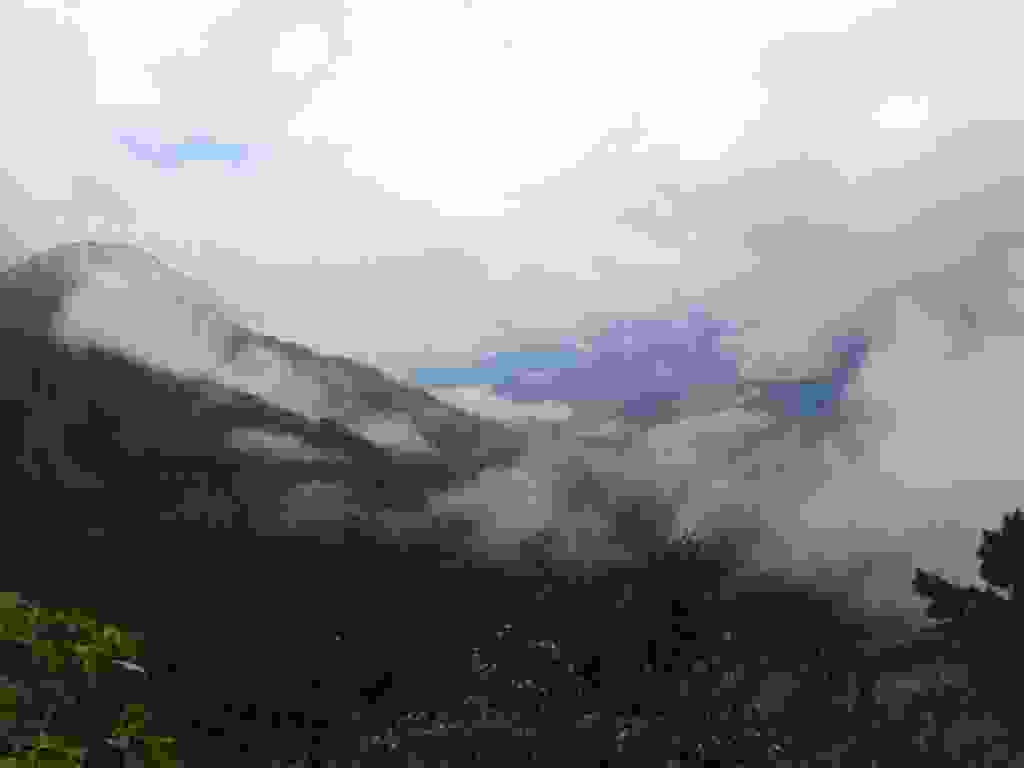
\includegraphics[width=\mywidth]{../wp-content/uploads/2015/11/wpid-oi000302-1024x768.jpg} } 
 \newline
 Côte nourriture plein de choses à tester, un thali pour commencer, à manger avec la main droite bien sûr \newline
 \newline
\centerline{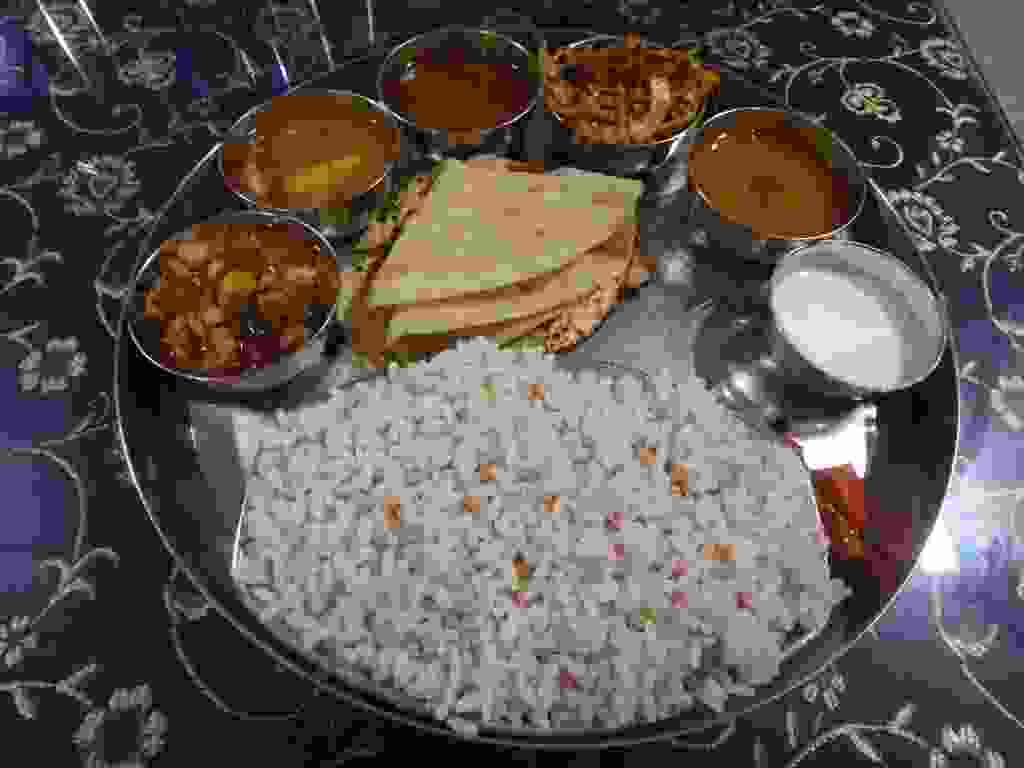
\includegraphics[width=\mywidth]{../wp-content/uploads/2015/11/wpid-oi000270-1024x768.jpg} } 
 \newline

\newpage
 
